%%% Note that the a4paper option is mainly intended so that authors in
% countries using A4 can easily print to A4 and see how their papers will
% look in print - the typesetting of the document will not typically be
% affected with changes in paper size (but the bottom and side margins will).
% Use the testflow package mentioned above to verify correct handling of
% both paper sizes by the user's LaTeX system.
%
% Also note that the "draftcls" or "draftclsnofoot", not "draft", option
% should be used if it is desired that the figures are to be displayed in
% draft mode.
%
\documentclass[10pt,conference]{IEEEtran}
% Add the compsoc option for Computer Society conferences.
%
% If IEEEtran.cls has not been installed into the LaTeX system files,
% manually specify the path to it like:
% \documentclass[conference]{../sty/IEEEtran}





% Some very useful LaTeX packages include:
% (uncomment the ones you want to load)

% *** MATH PACKAGES ***
%
\usepackage[cmex10]{amsmath}
% A popular package from the American Mathematical Society that provides
% many useful and powerful commands for dealing with mathematics. If using
% it, be sure to load this package with the cmex10 option to ensure that
% only type 1 fonts will utilized at all point sizes. Without this option,
% it is possible that some math symbols, particularly those within
% footnotes, will be rendered in bitmap form which will result in a
% document that can not be IEEE Xplore compliant!
%
% Also, note that the amsmath package sets \interdisplaylinepenalty to 10000
% thus preventing page breaks from occurring within multiline equations. Use:
%\interdisplaylinepenalty=2500
% after loading amsmath to restore such page breaks as IEEEtran.cls normally
% does. amsmath.sty is already installed on most LaTeX systems. The latest
% version and documentation can be obtained at:
% http://www.ctan.org/tex-archive/macros/latex/required/amslatex/math/





% *** SPECIALIZED LIST PACKAGES ***
%
%\usepackage{algorithmic}
% algorithmic.sty was written by Peter Williams and Rogerio Brito.
% This package provides an algorithmic environment fo describing algorithms.
% You can use the algorithmic environment in-text or within a figure
% environment to provide for a floating algorithm. Do NOT use the algorithm
% floating environment provided by algorithm.sty (by the same authors) or
% algorithm2e.sty (by Christophe Fiorio) as IEEE does not use dedicated
% algorithm float types and packages that provide these will not provide
% correct IEEE style captions. The latest version and documentation of
% algorithmic.sty can be obtained at:
% http://www.ctan.org/tex-archive/macros/latex/contrib/algorithms/
% There is also a support site at:
% http://algorithms.berlios.de/index.html
% Also of interest may be the (relatively newer and more customizable)
% algorithmicx.sty package by Szasz Janos:
% http://www.ctan.org/tex-archive/macros/latex/contrib/algorithmicx/




%\usepackage{array}




% *** PDF, URL AND HYPERLINK PACKAGES ***
%
%\usepackage{url}
% url.sty was written by Donald Arseneau. It provides better support for
% handling and breaking URLs. url.sty is already installed on most LaTeX
% systems. The latest version and documentation can be obtained at:
% http://www.ctan.org/tex-archive/macros/latex/contrib/url/
% Basically, \url{my_url_here}.




% *** Do not adjust lengths that control margins, column widths, etc. ***
% *** Do not use packages that alter fonts (such as pslatex).         ***
% There should be no need to do such things with IEEEtran.cls V1.6 and later.
% (Unless specifically asked to do so by the journal or conference you plan
% to submit to, of course. )


% correct bad hyphenation here

\usepackage[english]{babel}
\usepackage{graphicx, type1cm, lettrine}
\usepackage{graphicx}
\usepackage{epstopdf} %%package to overcome problem with eps in pdf files
\usepackage{cite}


\begin{document}


%
% paper title
% can use linebreaks \\ within to get better formatting as desired
% Do not put math or special symbols in the title.
% title actual
% Collaborative filtering: Techniques and Applications
\title{Recommendations for the Amazon Learning systems}
\title{Recommendations using Collaborative filtering and other techniques}
\title{Collaborative filtering using various techniques}
\title{Collaborative filtering: State of the Art and Trends}

% author names and affiliations
% use a multiple column layout for up to three different
% affiliations


\author{
\IEEEauthorblockN{Rahul Bali}
\IEEEauthorblockA{Department of Computer Science\\
Punjab Engineering College\\
Chandigarh, India\\
Email: rahulrdb18@gmail.com}
% email: rahulbali.mecse16@pec.edu.in
\and
\IEEEauthorblockN{Shilpa Verma}
\IEEEauthorblockA{Department of Computer Science\\
Punjab Engineering College\\
Chandigarh, India\\
Email: shilpaverma.pec@gmail.com}}

% email: shilpaverma.pec@gmail.com

% conference papers do not typically use \thanks and this command
% is locked out in conference mode. If really needed, such as for
% the acknowledgment of grants, issue a \IEEEoverridecommandlockouts
% after \documentclass

% for over three affiliations, or if they all won't fit within the width
% of the page, use this alternative format:
% 

% a kind of multiline comment
\iffalse

\author{\IEEEauthorblockN{Michael Shell\IEEEauthorrefmark{1},
Homer Simpson\IEEEauthorrefmark{2},
James Kirk\IEEEauthorrefmark{3}, 
Montgomery Scott\IEEEauthorrefmark{3} and
Eldon Tyrell\IEEEauthorrefmark{4}}
\IEEEauthorblockA{\IEEEauthorrefmark{1}School of Electrical and Computer Engineering\\
Georgia Institute of Technology,
Atlanta, Georgia 30332--0250\\ Email: see http://www.michaelshell.org/contact.html}
\IEEEauthorblockA{\IEEEauthorrefmark{2}Twentieth Century Fox, Springfield, USA\\
Email: homer@thesimpsons.com}
\IEEEauthorblockA{\IEEEauthorrefmark{3}Starfleet Academy, San Francisco, California 96678-2391\\
Telephone: (800) 555--1212, Fax: (888) 555--1212}
\IEEEauthorblockA{\IEEEauthorrefmark{4}Tyrell Inc., 123 Replicant Street, Los Angeles, California 90210--4321}}

I don't want this to happen
\fi


% make the title area
\maketitle

% As a general rule, do not put math, special symbols or citations
% in the abstract
\begin{abstract}
	The world has seen much change in ways which recommendations were made since the first arrival of the collaborative filtering in providing recommendations. The paper below describes the various advancements and the changes in the field of the collaborative filtering. The state of the art recommendations engines have been described with their best chances of survival. Certain trends have also made it to this work.
\end{abstract}


% no keywords




% For peer review papers, you can put extra information on the cover
% page as needed:
% \ifCLASSOPTIONpeerreview
% \begin{center} \bfseries EDICS Category: 3-BBND \end{center}
% \fi
%
% For peerreview papers, this IEEEtran command inserts a page break and
% creates the second title. It will be ignored for other modes.
\IEEEpeerreviewmaketitle


%% keywords for the writing.
%%% information overload
%%% computer-human interaction
%%% 
\section{Introduction}
% no \IEEEPARstart
\lettrine[lines=2, findent=1pt, nindent=0pt]{W}e are living in the age of technology and ``computer-human interaction''. In fact computer-human interaction has gone past the human-human interaction.[citation needed] The day is not far from when we will be having complete human-computer interface.
The interest in this area of machine learning is at its all time high and the applications in the real world scenarios are helping much users to deal with information overload.


\begin{figure*}
\centering
        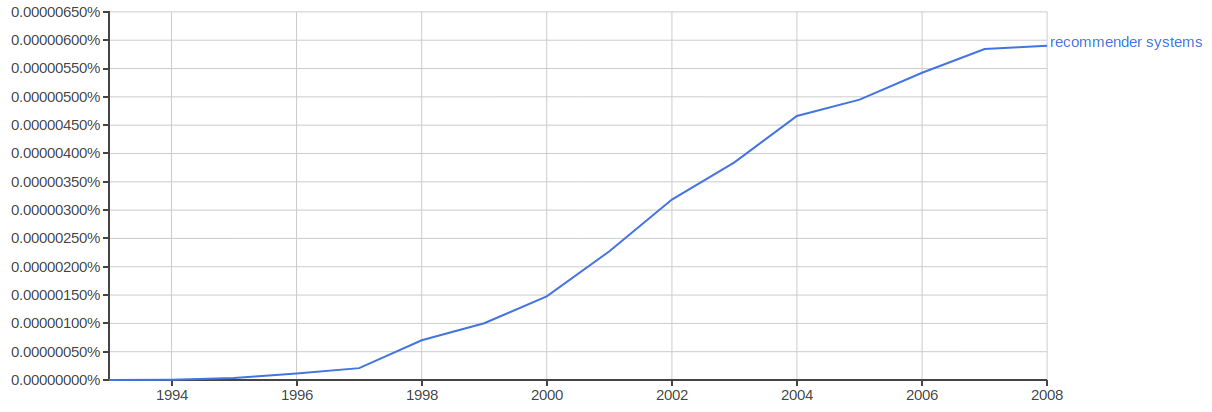
\includegraphics[width=\textwidth]{images/history-use}
    \caption{used}
    \label{fig:verticalcell}
\end{figure*}

[ngram]
%(https://books.google.com/ngrams/graph?content=recommender+systems&year_start=1960&year_end=2017&corpus=15&smoothing=3&share=&direct_url=t1\%3B\%2Crecommender\%20systems\%3B\%2Cc0)
The recommender systems have been around for more than a decade and has only seen the increase in popularity and applications.
Current state of recommender system make us proud for doing research efforts. This research is an addition to the committed work of the authors around the globe for recommendation engines.

Recommender systems are considered as gadgets and programing building association that is used for producing points of interest recommendation to the clients, and in addition to help them in the strategy of basic leadership.One of the regular recommender systems procedures is collaborative filtering (CF). The essential thought of CF is the extraction of data about the old conduct or conclusions to client that exist in the public arena, any components where expected that the present client of the framework are probably going to have readiness to be chosen, or like his taste. The CF approach takes a grid which is given to the client just by evaluating the data sources and a comparable estimate for the accompanying sorts of yield. Crafted by CF is to give evaluations of the present number of dynamic client input and recognize different clients.

At that point, it accomplishes correlation procedure to get to the nearest person for the active user benevolent for any comparative inclinations with the active user. These days, Collaborative filtering can be grouped into three principal classifications as appeared in Figure l.There is a solid assemblage of research that has been directed in these three fundamental methods model-based, memory based and hybrid based strategies. In memory based model, the framework tries to discover clients who take after the present dynamic client inclinations and is used to foresee the present dynamic client inclinations. That is, memory-based technique is a compelling way and simple to actualize, which is utilized: neighborhood-based CF, thing based, client based and top-N. As to the idea of the model based, there is a rendition to assemble a model based on the assessment information or a portion of the extraction of infonnation from the dataset and used to assemble a model to make proposals without the need of utilizing the informational collection at once. While hybrid based is a blend between the two past strategies, it takes preferences of the highlights of memory and keep away from hindrances of the highlights of the model. The use of the CF is utilized as a part of various investigations taking care of the collaborative filtering in numerous fields, for example, internet business, promoting , e-Learning , social organizing locales and also in the advertising of books, motion pictures furthermore, music, daily paper, TV programs, and benefit focuses that incorporate travel, tourism, Customer Relationship Management, machine learning, and systems offers administrations.


This paper gives a review of the recommender framework and additionally to exhibit the utilization of the collaborative filtering calculation. In addition, an alternate model of CF calculations has been talked about and that probably the most critical logical papers distributed around there have been audited.

This paper is divided into certain segments as follows. Segment 2 plots the recommender systems strategies. Segment 3 gives a review of collaborative filtering approaches. The memory based arrangement is displayed in Section 4. Segment 5 exhibits the hybrid based collaborative filtering models. Area 6 features the improvement of the collaborative filtering techniques. A few issues, qualities and difficulties of the collaborative filtering are audited in Section 7. Area 8 gives an assessment measurements of the collaborative filtering systems. Exchange and finish of ebb and flow open research issues are given in Sections 8 and 9 individually.

\cite{su2009survey}
\cite{zuva2012survey}
\cite{herlocker2004evaluating}
\cite{linden2003amazon}
\cite{adomavicius2005toward}
\cite{park2012literature}


\section{Recommender Systems Techniques}
A few techniques have been proposed for use in recommender systems. A few examinations sort recommender systems in perspective of their technique with proposal in three kinds: content-based, collaborative, and hybrid procedures differentiated to their partners which have been characterized into four classes : Content based Filtering (CBF), knowledge based (KBF), Collaborative filtering (CF) and Hybrid filtering (HF) [4].

\subsection{Content Based Filtering(CBF)}
CBF approaches recommend items that are similar in content of the items that the user liked in the past or match to the attributes of the user.

CBF approaches prescribe things that are comparable in substance to the things that the user enjoyed previously or match to the properties of the user [5]. In content based filtering technique, every thing is spoken to by an element vector or a characteristic profile. The component holds numeric or ostensible esteems speaking to specific parts of the thing, for example, shading, cost, and so forth. An assortment of (dis) closeness measures between the component vectors might be utilized to ascertain the comparability between two things. The Euclidean or cosine (dis) comparability calculations can be utilized as in conditions (1) and (2) [4].

Where x and y are vectors of things with n components in them, dissim (x,y) and sim(x,y) measure the separation separated and closeness individually. The (dis) similarty values are then used to acquire a ranked list of recommended items. These techniques are relying upon information retrieval, and they can give recommendations in any area. In content based strategies, when the items are spoken to as an arrangement of highlights in a legitimate and clear way, at that point the framework can function admirably. Content-based recommender systems make proposals through substance examination of printed data, for instance, reports, thing portrayals, newsletter, URLs, web logs, profiles for users' needs, inclinations, tastes, and discover consistency in the content.

\textbf{here are the bold stuff}

\subsection{Knowledge based filtering (KEF)}
Knowledge based filtering approaches are acclaimed in the way that they have utilitarian learning. These strategies have learning concerning how a specific thing fulfills a specific client require, in this way, one can think about the connection between the need and conceivable proposal. Learning based methodologies have comparably an itemized portrayal of the client's needs [3].


\subsection{Hybrid filtering Techniques}
Hybrid filtering alludes to a mix of at least two approaches; the objective of this mix is to defeat the absences of one approach with other one. The blend of collaborative filtering methodologies and substance based deliver separated rank's arrangements of suggestions and consolidate them to build up the new proposal result.

These hybrid methodologies contain the substance of the thing, the appraisals of clients, content-based filtering, and statistic data. One well known case of these hybrid systems is weighted and exchanging. In a weighted hybrid framework, the score of a suggested thing can be processed from the accessible outcomes based on accessible proposal approaches. Then again, exchanging hybrid framework utilizes a few gauges to switch among suggestion approaches. Collaborative filtering might be converged with other strategy attempting to escape from the increase issue. Study [2] applied 'Determination operator', utilized hybrid of CF and substance based filtering. Another investigation, for example, in, additionally connected hybrid method for proposal and utilized a greater amount of the accessible data and in this manner has more exact suggestions.
Having exhibited above sections on recommender systems strategies can be utilized for some, applications based on the application space, which can decide the reasonable procedure. In this paper, we will center around the CF calculation. 

\section{Collaborative Filtering Approaches}
Generally, CF methodologies can be ordered into two classes: memory based and model based strategy. The memory based strategy requires all appraisals, things and clients to be put away in a memory. Then again, model based techniques have a tendency to make an outline of evaluations designs offline \cite{sarwar2001item}.

The Probabilistic CF techniques are based on a basic probabilistic model while non-probabilistic CF strategies are not based on probabilistic model [3]. One of the notable CF non-probabilistic is the closest neighbor strategy. Closest neighbor systems can be separated into two classes; thing based closest neighbor and client based closest neighbor [4]. 

\subsection{Model based CF}
Model based CF techniques foresee the dark appraisals following taking in a model from the fundamental data utilizing machine learning or measurable techniques [5]. Model-based
CF techniques, for example, dependence systems, Bayesian and bunching model should be perceived to handle those deficiencies about memory-based CF approaches. Model-based strategies comprises of Bayesian classifiers, backslide based techniques and group based CF. The idea of the model based CF forms is to assemble a model based on the assessment information, or is to construct a portion of the extraction of data from the information gathering and dataset that utilized and to influence proposals without using to the dataset at once. 

\subsection{Memory based CF}
Memory based CF techniques intend to utilize past information to foresee the obscure rating rely upon some heuristic [5], They are working over the whole client database to anticipate the outcomes. We can find that the normally memory based strategies are based on the idea of closest neighbors, utilizing an assorted variety of separation measures. The procedure of the foreseeing evaluations through alluding to clients which their appraisals are like the questioned client based on neighborhood-based strategies, which are basic memory-based CF approaches. As to the creation of memory-based CF techniques expectation, an example of the client? thing database is utilized. Every client has a place with a gathering of individuals that have comparable interests. The memory based CF has a few highlights, for example, clear up the outcomes. As it were, memory based CF is viewed as an essential part of suggestion systems, convenience, encouraging new information effortlessly, autonomy substance of components that are prescribed to grow the extent of a decent appraising with the regular components. Furthermore, the disservices of memory based CF is the issues on focuses clear and moderate. Likewise, the trouble of improvement Particularly with regards to the genuine systems that creates suggestions continuously based on expansive datasets [3]. 

\subsection{Memory versus Model Based}
Collaborative filtering calculates certain similarities between neighbours in memory based CF. This technique is called memory based; the database of segments will be stacked in working memory and utilized specifically in order to generate recommendations. In contrast to this technique, there is the model based strategy, in which a model is adjusted and used to used to create recommendations. Model based strategy creates a model in offline environment, and recommendations take place in the online system almost immediately. Model Based algorithms were huge part of the final solution for the winning team on the Netflix Million Dollar prize 2006. The winning solution had over 100 different techniques and methodologies of a weighted ensemble, the major algorithms were Model based Matrix Factorization.

\section{Memory Based Classification}
As we said before, the memory based CF strategies work based on the past information and anticipate rating, the normal memory based CF techniques are based on the idea of closest neighbors. Memory based CF strategies for the most part rely upon client has a place of a gathering of individuals who have comparative interests. CF approaches which follow the same ideas of the memory based divided into the following approach.

\subsection{Item based}
Item based collaborative filtering is a sort of model based technique for making suggestions. There are two stages in thing based collaborative filtering. Initially, discover the likenesses between things that are processed by utilizing one of the number closeness measures. Furthermore, surveyed likeness esteems by utilizing foresee appraisals for obscure thing. Thing based closest neighbor strategies are transpose of the client based closest neighbor techniques. Be that as it may, it can make expectations rely upon similitudes among items. 

The cosine based similarity strategy is regular approach to figure out the similarity between items, as should be obvious in equation(3).

\begin{equation}
	ItemSim(x, y) = \sum_{u \in U} ({R_{u,i} - \overline{R}_u}) ({R_{u,j} - \overline{R}_u}) / ({R_{u,j} - \overline{R}_u})
\end{equation}


\subsection{User based}
User based collaborative filtering techniques for decide the closeness of the client by breaking down the components partook in the vote between the client and that of the client utilizes the similitudes and anticipated weight keeping in mind the end goal to evaluate the imperative rating of the client on the effectiveness of the component. The Pearson connection efficient similitude is the most used to register comparability strategies as given in condition (5) [4].

\textbf{some portion missing here-- like equations}

\subsection{Item vs User based}
From the previous sections, we have understood that the kinds of mempry based collaborative filtering methods use dimensions of the user-item rating matrix to find similarities.
Each one has its own separate behaviour and advantages.


\section{HYBRID BASED COLLBAORATIVE FILTERING}
In this kind of model for the collaborative filtering, memory based and model based structures are used to make the recommendations and predictions for the user. It has been in the use for much time now, it takes the advantages of the better portions of the two methods and leaves what is not very useful at different stages of the recommendations.

\section{Enhance the Collaborative Filtering Approach}
In Collaborative filtering techniques, many type of success in different types of domains, much more improvements are still required for enhancement of the Collaborative filtering.
The study in [7] recommended a hybrid method that considers clients' buy arrangements after some time. This strategy upgrades the nature of suggestions to give proposals based on client groups. The creators presented a best in class and scientific classification of savvy recommender operators on the understudy et on various systems of suggestions framework. In examine [6], machine learning procedures utilized as an important apparatus for accomplishment a target comprehension of how esteems are installed in advancements are displayed. 

Another study as in \cite{ekstrand2011collaborative} exhibited a novel technique to non-local versatile nonparametric filtering for the image modeling. However, an study [2] suggested an upgraded CF strategy by utilizing a genetic algorithm for getting ideal likeness capacities to acquire better quality and faster outcomes as a hybrid technique. 
Also,[2] introduced collaborative filtering strategy with upgrade the recommendation quality emerging from user made tags to overcome a portion of the constraints in CF systems.

\section{Challenges of CF}
Recommendations used for the large large online e-commerce companies like eBay, Flipkart and Amazon(India) have created a challenging environment. A recommender system is expected to provide with faster and accurate recommendations that will attract the interest of customers and yield profits for the companies. For CF techniques, handling the challenges to produce high quality predictions or recommendations which can describe the characteristics of the CF techniques.

\subsection{Scalability}
Traditionally, CF techniques will suffer genuine scalability issues if quantities of existing clients and things develop colossally. For example, with a huge number of clients (M) and a huge number of distinct catalog items (N), a CF algorithm with the complexity of O(n) is now too large. Besides, numerous systems need to respond immediately to online necessities and make recommendations for all users regardless of their purchases and ratings history, which request a high versatility of a CF framework [3].

\subsection{Synonymy}
The synonym word is a likelihood of some of the same or exceptionally comparable items to have diverse names or entries. Numerous recommender systems are unable to find this inactive affiliation and therefore treat these items in an unexpected way. For example, the apparently unique things "youngsters motion picture" and "kids film" as they seem to be, indeed, a similar thing, yet the memory-based CF techniques would discover no match between them to figure comparability. The predominance of equivalent words lessens the suggestion execution of CF approaches [3].

\subsection{Data Scatter}
In fact, many commercial recommender systems are used to evaluate very large product data sets. The user item matrix utilized for CF approach will consequently be extremely meager and that exhibitions of the forecasts or proposals of the CF systems are tested [3].

\subsection{Gray Sheep}
The users whose opinions do not consistently agree or disagree with group individuals and hence don't profit from CF. Then again, the contrary gathering whose particular tastes make suggestions almost incomprehensible had known as black sheep. Despite the fact that this is a failure of the recommender system, non-electronic recommenders additionally have huge problems in these cases, therefore, black sheep is a satisfactory failure.

\subsection{Shilling Attacks}
In the world of competitive business models, recommendations may be biased toward people's own profit. People may recommend positive recommendations of own product and negative recommendations for the competitors products. This type of behaviour must be discouraged in the recommender systems and precautions must be taken against it.[3]


\section{Evaluation Metrics}

The evaluation metrics are of huge importance in the field of recommender systems. Outcome of any model or systems design for recommender system needs to be evaluated for performance. The performance can be measured in terms of many different evaluation metrics. The choice of evaluation metrics depends on the application area of the CF algorithms. Most commonly used metrics are: Mean Absolute Error (MAE), Normalized Mean Absolute Error (NMAE), Root Mean Squared Error (RMSE) and ROC sensitivity and the Area under ROC Curve(AUC).

\textbf{some portion missing here-- like equations}

\section{Conclusion}
Collaborative filtering techniques emphasize the accomplishment of utilizing recommender systems strategy in various regions of research. In this paper, we presented the fundamental recommender systems strategies. At that point, the fundamental classifications of collaborative filtering strategies have been presented which incorporate; memory-based, model based, and hybrid CF technique that consolidate CF with other recommender framework strategies. In addition, a few cases of specified CF systems have been given. The paper also features a few proposals to upgrade CF technique and utilizing the improvement in various application applying CF strategy. The assessment measures have been talked about also. This examination seems to propose as well as show that the more far off future may have a place with different calculations, it enhances the recommender framework.



\newpage
\bibliographystyle{IEEEtran}
\bibliography{references}




% that's all folks
\end{document}


